\documentclass[notes]{beamer}

\usetheme{Darmstadt}
\usepackage{lmodern}% http://ctan.org/pkg/lm
\usepackage{amsthm,amstext,amsfonts,bm,amssymb}

\mode<presentation>
%\useoutertheme{smoothbars}
\useinnertheme[shadow=true]{rounded}
\usecolortheme{whale}
\useoutertheme{split}
\usefonttheme[onlysmall]{structurebold}
\usefonttheme{professionalfonts}
\usepackage{amssymb}
\usepackage{verbatim}
%\setbeamertemplate{footline}[frame number]
\mode
<all>

\usepackage{algorithmic}
\usepackage{algorithm}
\renewcommand{\algorithmicrequire}{\textbf{Input:}}
\renewcommand{\algorithmicensure}{\textbf{Output:}}
\newcommand{\algorithmiclocal}{\textbf{Local Variables: }}
\newcommand{\LOCAL}{\item[\algorithmiclocal]}
\newcommand{\algorithmicsend}{\textbf{send }}
\newcommand{\algorithmicreceive}{\textbf{receive }}
\newcommand{\SEND}{\algorithmicsend}
\newcommand{\RECEIVE}{\algorithmicreceive}
\newcommand{\true}{\textbf{true}}
\newcommand{\false}{\textbf{false}}

\newcommand{\red}{\textcolor{red}{red }}
\newcommand{\blue}{\textcolor{blue}{blue }}
%\newcommand{\<--}{$\longleftarrow$}
%\newcommand{\<-}{$\leftarrow$}
%\newcommand{\-->}{$\longrightarrow$}
%\newcommand{\->}{$\rightarrow$}

% % % % % margin notes % % % % % %
%\usepackage[margin=1cm]{caption}
%\usepackage[colorinlistoftodos,prependcaption
%%,textsize=tiny
%]{todonotes}

%\reversemarginpar
%\newcommand\todoil[1]{\todo[inline]{ #1}}
\newcommand\todoil[1]{ {\color{red}\textit{\textbf{TODO:} #1}} }
% % % % % % % end % % % % % % % %

%%%%%%%% Packages for drawing diagrams %%%%%%%%%%%%%%%
\usepackage{tikz,ifthen}
\usetikzlibrary{arrows,automata,positioning }
\tikzstyle{block}=[rectangle, draw, thin, inner sep=3pt, text centered, 
%drop shadow, 
fill=orange!20!yellow!20] 
\tikzstyle{pre}=[<-,shorten <=1pt,>=stealth']
\tikzstyle{post}=[->,shorten >=1pt,>=stealth'] 
\tikzstyle{bi}=[<->,shorten >=1pt,shorten <=1pt,>=stealth'] 
\tikzstyle{every initial by arrow}=[initial text={},initial distance=1em,post]
%\tikzstyle{every state}=[minimum size=0.4cm,drop shadow,fill=orange!20!yellow!20]
\tikzstyle{transition}= [post,shorten >=1pt,node distance=2cm, inner sep=2pt,bend angle=20]
\tikzstyle{box}=[rectangle,draw=black, thick, inner sep=3pt, text centered]

%Hodai part
%\usepackage{tikz}
\usetikzlibrary{shapes.geometric, arrows, automata, positioning}
\tikzstyle{recNode} = [rectangle, minimum width=2cm, minimum height=1cm, text centered, rounded corners=0.1cm, draw=black]
\tikzstyle{recNodeB} = [recNode, draw=blue, fill=blue!10,text=blue!20!black]
\tikzstyle{recNodeG} = [recNode, draw=red, fill=red!10,text=red!10!black]
\tikzstyle{eNode} = [minimum height=1cm, text centered,text=blue!20!black]

\tikzstyle{arrow} = [thick,->,>=stealth,draw=black]
\tikzstyle{arrowB} = [thick,->,>=stealth,draw=blue]
\tikzstyle{arrowG} = [ultra thick,->,>=stealth,draw=red, dashed]

%%%%%%%% end %%%%%%%%%%%%%%%

\usepackage[english]{babel}
%\usepackage{graphicx}
\usepackage{amssymb}
%\usepackage{caption}
%\usepackage{MnSymbol}

\RequirePackage{pgf,pgffor}

\usepackage[mathcal]{euscript}

\newcommand{\commentOut}[1]{}
\newcommand{\uncomment}[1]{#1}

\newcommand{\buchi}{B\"uchi }


\def\A{{\cal A}}
\def\B{{\cal B}}
\def\C{{\cal C}}
\def\D{{\cal D}}
\def\E{{\cal E}}
\def\F{{\cal F}}
\def\G{{\cal G}}
\def\H{{\cal H}}
\def\I{{\cal I}}
\def\J{{\cal J}}
\def\K{{\cal K}}
\def\L{{\cal L}}
\def\M{{\cal M}}
\def\N{{\cal N}}
\def\O{{\cal O}}
\def\P{{\cal P}}
\def\Q{{\cal Q}}
\def\R{{\cal R}}
\def\S{{\cal S}}
\def\T{{\cal T}}
\def\U{{\cal U}}
\def\V{{\cal V}}
\def\W{{\cal W}}
\def\X{{\cal X}}
\def\Y{{\cal Y}}
\def\Z{{\cal Z}}

\usepackage{graphicx}
\usepackage{theorem} 

\graphicspath{{./img/}}  

\newcommand{\old}[1]{{}}
\AtBeginSubsection[]
{
	\begin{frame}<beamer>{Outline}
		\tableofcontents[currentsection,currentsubsection]
	\end{frame}
}

% % % % % % % % % % % % the title page % % % % % % % % % % % %

\title[Reactive Scheduling]{Reactive Scheduling of Computational Resources in Control Systems}
\author[Hodai Goldman]{Hodai Goldman}
\institute{
    { Ben-Gurion University of the Negev\\
    Department of Computer Science}
}
\date{January 1, 2018}


\begin{document}

\frame{\titlepage}

\frame{\tableofcontents}


\section{Automata-based Scheduling}
\subsection{motivation}
\def\tikzFeadback{
     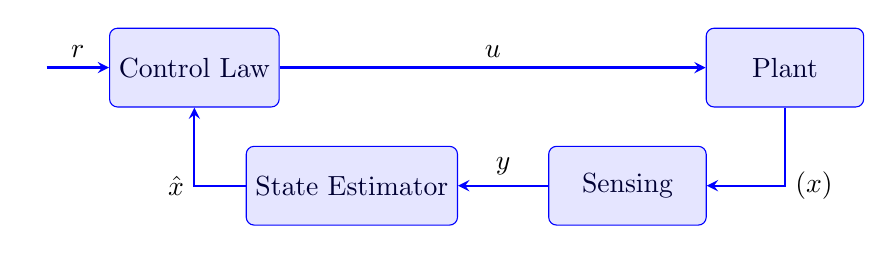
\begin{tikzpicture}[node distance=1.5cm]
         \node (in) [eNode] {};
         \node (control) [recNodeB, right of=in, xshift=0.5cm] {Control Law};
         \node (sys) [recNodeB, right of=control, xshift=6cm] {Plant};
         \node (sensor) [recNodeB, below of=sys, xshift=-2cm] {Sensing};
         \node (estimator) [recNodeB, below of=control, xshift=2cm] {State Estimator};
         
         \draw [arrowB] (in) -- node[above] { $r$} (control);
         \draw [arrowB] (control) -- node[above] { $u$} (sys);
         \draw [arrowB] (sys) |- node[right] { ($x$)} (sensor);
         \draw [arrowB] (sensor) -- node[above] { $y$} (estimator);
         \draw [arrowB] (estimator) -| node[left] { $\hat{x}$} (control);
     \end{tikzpicture}
}
\def\myPerionTable{
    \begin{tabular}{|c c c|} 
        \hline
        Task & Period & Deadline \\ 
        \hline
        Check for obstacles & 10ms & 1.5ms \\ 
        %\hline
        Check GPS position & 10ms & 0.5ms \\
        Control Law & 2ms & 0ms \\
        \multicolumn{3}{|c|}{$\cdots$}\\
        \hline
    \end{tabular}
}

    \frame{
        \frametitle{An control problem example}
        \todoil{present the example: robot moving in root with obstacles, mission 1: avoid obstetrical(camera), mission 2: follow the guiding root(GPS)}
        \begin{figure}
             
        \end{figure}
    }	
     \frame{
         \frametitle{The Traditional Solution}
         \begin{center}
             \tikzFeadback
         \end{center}
         \begin{center}
             {\Huge \textbf{+}}
         \end{center}
         \begin{block}{Constant time steps + periodic tasks}
             \begin{center}
                 \todoil{{time steps\\ figure}} + 
                 \myPerionTable
             \end{center}
         \end{block}
     }	
    \frame{
        \frametitle{The Main Software Design Problems}
        \begin{center}
            \myPerionTable
        \end{center}
        \begin{block}{The design problems from our point of view}
            \begin{itemize}
                \item \textbf{All the tasks are highly coupled}: \textit{any change or addition of some task require to consider all other tasks requirements}
                \item \textbf{Static and inefficient scheduling}: \textit{the table is defined for the worst case} \todoil{talk about related work on this direction}
                \item \textbf{No consideration of the environmental conditions}: it is a cyber-physical system after all
            \end{itemize}
        \end{block}
    }
     
    \frame{
        \frametitle{The Goal}
        \begin{block}{}
            In this thesis we design an \textbf{reactive} scheduling framework for real-time systems
        \end{block}
        \begin{block}{Required features: \commentOut{of the scheduling framework for real-time systems}}
            \begin{itemize}
                \item \textbf{Independent} and \textbf{composable} requirements
                \item \textbf{Control objective based} requirement interface
                \item Environment \textbf{adoptive} scheduler
            \end{itemize}
        \end{block}
    }
     
\subsection{Component-based Architecture}

\def\tikzArch{
    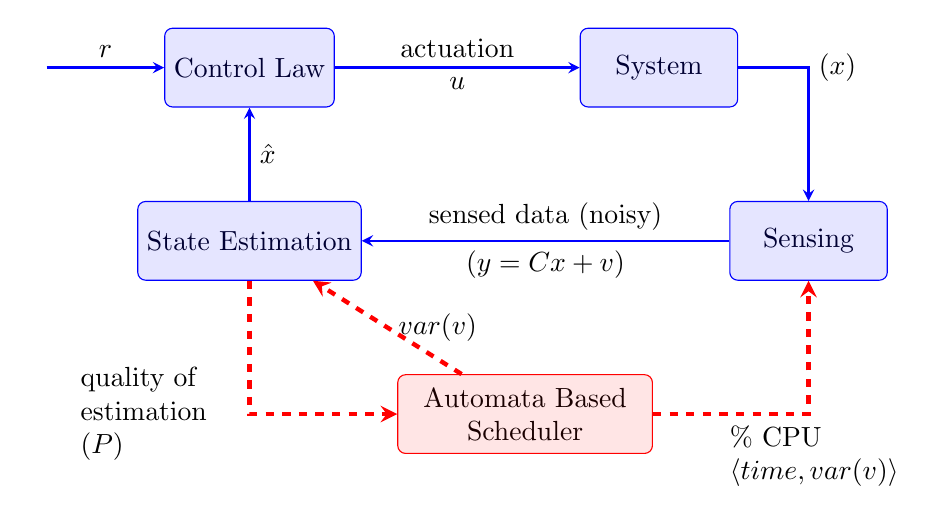
\begin{tikzpicture}[node distance=1.2cm]
    \node (in) [eNode] {};
    \node (control) [recNodeB, right of=in, xshift=1.5cm] {Control Law};
    \node (sys) [recNodeB, right of=control, xshift=4cm] {System};
    \node (sensor) [recNodeB, below of=sys, xshift=1.9cm, yshift=-1cm] {Sensing};
    \node (estimator) [recNodeB, below of=control, yshift=-1cm] {State Estimation};
    \node (sched) [recNodeG, below of=estimator, yshift=-1cm, xshift=3.5cm, text width=3cm] {Automata Based Scheduler};
    
    \draw [arrowB] (in) -- node[above] {$r$} (control);
    \draw [arrowB] (control) -- node[above] {actuation} node[below] {$u$} (sys);
    \draw [arrowB] (sys) -| node[right,text width=1cm] {($x$)} (sensor);
    \draw [arrowB] (sensor) -- node[above] {sensed data (noisy)} node[below] {$(y = Cx +v$)} (estimator);
    \draw [arrowB] (estimator) -- node[left,text width=2cm] {} node[right] {$\hat{x}$} (control);
    
    \draw [arrowG] (estimator) |- node[left,text width=2cm] {quality of estimation ($P$)} (sched);
    
    \draw [arrowG] (sched) -| node[below,text width=2cm] { \% CPU $\langle time,var(v) \rangle$} (sensor);
    %\draw [arrowG] (sched) -| node[right] {$\langle time,var(v) \rangle$} (sensor);
    
    \draw [arrowG] (sched) --  node[right] {$var(v)$} (estimator);
    
    \end{tikzpicture}
}

\frame{
    \frametitle{The Proposed Architecture}
    
    %\begin{center}
    \begin{columns}
        \begin{column}{5cm}
            \scalebox{0.5}{
                \tikzArch
            }
        \end{column}
        \hfill
        {\huge +}
        \hfill
        \begin{column}{4cm}
            \todoil{figure of automata}
        \end{column}
    \end{columns}
    %\end{center} 
}

\frame{
    \frametitle{The Proposed Architecture - The System Design}
    {\todoil{Explain that the scheduler is involve in the control loops}}
    \begin{center}
        \scalebox{0.9}{
            \tikzArch
        }
    \end{center} 
}

\frame{
    \frametitle{The Proposed Architecture - The Specification interface}
    {\todoil{explain the advantage of automata}}\\
    \todoil{maybe add a word about RTcomposer and GameComposer}\\
    \begin{center}
        \todoil{Figure os guided automata}
    \end{center} 
}


\subsection{\buchi Games Interface}
    \todoil{\buchi game remainder}
\subsection{Sub-Summery: Component Definition}
    \todoil{technical}
    
    
\section{Integration with Kalman}
\subsection{Guiding Concept}
    \todoil{Explain the concept of estimate the errors}
\subsection{Guided Tour Simulation}
    \todoil{the simulation}
    

\section{Experiment with real-life case study}
\subsection{The mission}
    \todoil{1. mission definition}
    \todoil{2. scheduling objectives}
    \todoil{3. how we review the results (the $x$ axis)}
    \todoil{4. add a video}
\subsection{Simplifying the Kalman filter with complementary filter}
    \todoil{1. why not Kalman}
    \todoil{2. how we use complementary filter}
    \todoil{3. the linearize model in $x$ / roll axis}
    \todoil{4. update state (equations)}
\subsection{Results}
    \todoil{the automata and their results}

\section{Related Work}
    \todoil{review of similar papers: A table with few papers}

% % % % Conclusion  % % % %
% % % % % % % % % % % % % %
\section{Conclusion}
\subsection{Conclusion}
    \todoil{instead of with Related Work}
\frame{
%        \frametitle{Thanks}
\begin{center} 
    \Huge{Thanks} 
\end{center}
}
\end{document}
